\documentclass{article}
\usepackage{tikz}
\usetikzlibrary{automata,positioning}

\begin{document}

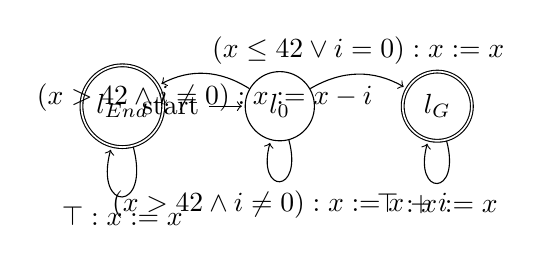
\begin{tikzpicture}[shorten >=1pt,node distance=2cm,on grid,auto]
    \node[state,initial] (l0) {$l_0$};
    \node[state,accepting] (lEnd) [left of=l0] {$l_{End}$};
    \node[state,accepting] (lG) [right of=l0] {$l_G$};

    \path[->]
        (l0) edge [loop below] node {$(x > 42 \land i \neq 0): x := x + i$} ()
        (l0) edge [bend left] node {$(x \leq 42 \lor i = 0): x := x$} (lG)
        (l0) edge [bend right] node {$(x > 42 \land i \neq 0): x := x - i$} (lEnd)
        (lEnd) edge [loop below] node {$\top : x := x$} ()
        (lG) edge [loop below] node {$\top : x := x$} ();
\end{tikzpicture}

\end{document}